\label{cap:appendice c}
\chapter{Descrizione dettagliata delle interfacce}
In questa sezione vengono descritte tutte le interfacce della web-app e i servizi utilizzati. La descrizione delle principali interfacce sono reperibili alle sezione 4.2.
\subsubsection{Menù}
Viene mostrata il menù del ristorante che comprende tutte le categorie e le loro piatti.\\
\textbf{Funzionalità:}
\begin{itemize}
    \item L'utente può aumentare la quantità di un piatto per aggiungerlo o aumentare la sua quantità nell'ordine del tavolo;
    \item L'utente può diminuire la quantità di un piatto per rimuoverlo o diminuire la sua quantità nell'ordine del tavolo;
    \item L'utente può visualizzare il piatto in modalità dettaglio per dare una recensione al piatto o inserisce una nota per il piatto;
    \item L'utente può aggiungere il piatto nella lista dei preferiti o rimuoverlo dalla lista.
\end{itemize}
\begin{figure}[H]
    \centering
    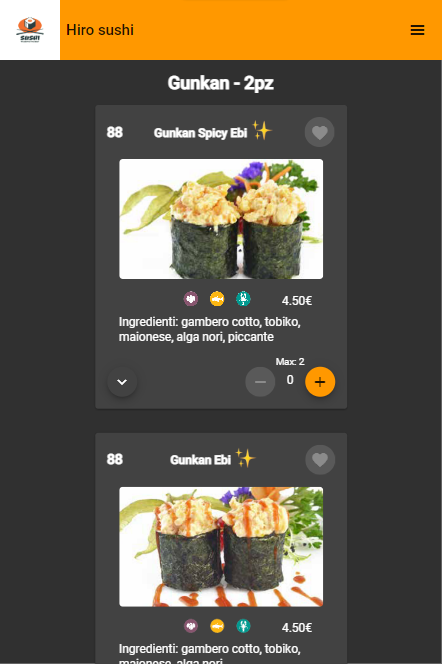
\includegraphics[scale=0.4]{menu.png}
    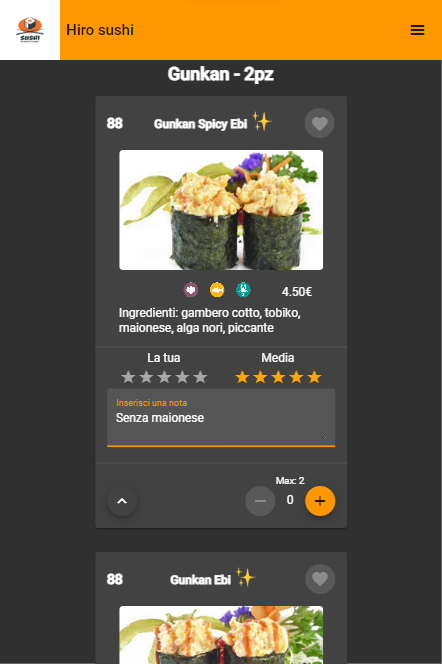
\includegraphics[scale=0.4]{menu2.png}
    \caption{Maschera menù di SushiLab}
\end{figure}


\subsubsection{gestione del tavolo}
Viene mostrata la maschera di gestione del tavolo.\\
\textbf{Funzionalità:}
\begin{itemize}
    \item L'utente può creare una sessione di tavolo;
    \item L'utente può andare al form per unire ad una sessione.
\end{itemize}
\begin{figure}[H]
    \centering
    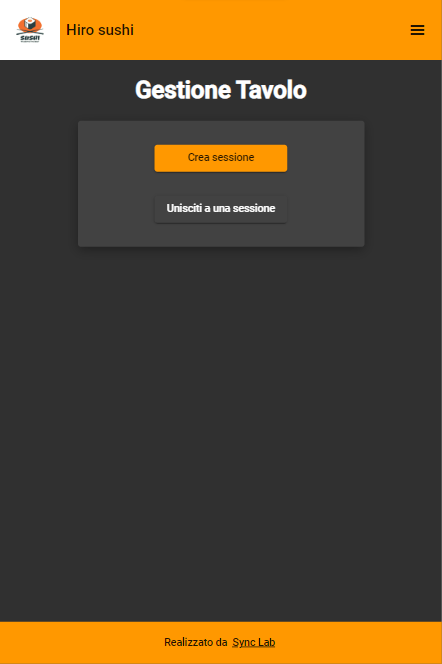
\includegraphics[scale=0.4]{gestione tavolo.png}
    \caption{Maschera gestione del tavolo di SushiLab}
\end{figure}


\subsubsection{Unisci sessione}
Interfaccia tramite la quale è possibile unire ad una sessione di tavolo.\\
\textbf{Funzionalità:}
\begin{itemize}
    \item L'utente può  unirsi ad una sessione inserendo il codice di sessione se il codice non rispetta la validazione del form non si abilita il bottone unisci;
    \item L'utente può tornare nella pagina gestione del tavolo.
\end{itemize}
\begin{figure}[H]
    \centering
    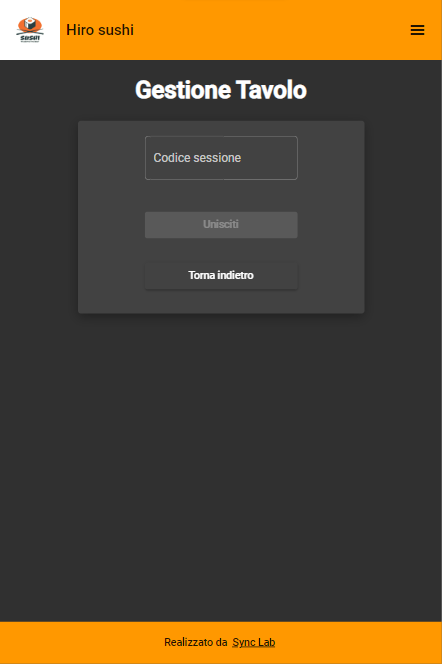
\includegraphics[scale=0.4]{unisci.png}
    \caption{Maschera unisci sessione di SushiLab}
\end{figure}


\subsubsection{QR-code tavolo}
Viene mostrata il QR-code del tavolo che permette agli altri utenti che si trovano sullo stesso tavolo dell'utente di unirsi.\\
\textbf{Funzionalità:}
\begin{itemize}
    \item L'utente può uscire dalla sessione premendo il bottone esci dalla sessione.
\end{itemize}
\begin{figure}[H]
    \centering
    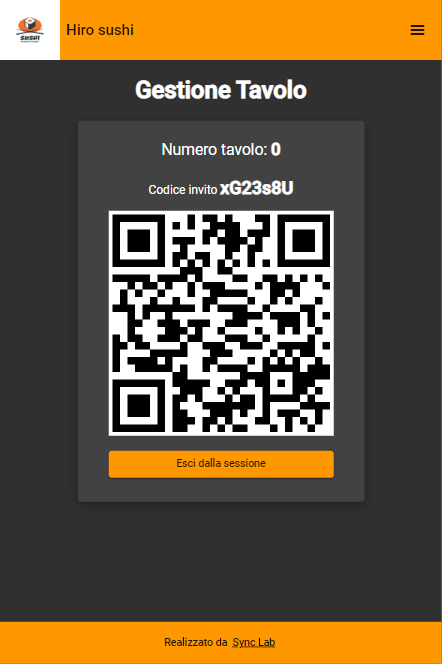
\includegraphics[scale=0.4]{gestionetavolo2.png}
    \caption{Maschera QR-code tavolo di SushiLab}
\end{figure}


\subsubsection{lista degli ordini del tavolo}
Viene mostrato la lista degli ordini della sessione del tavolo in cui si trova l'utente.\\
\textbf{Funzionalità:}
\begin{itemize}
    \item L'utente può spostare la lista in arrivo;
    \item L'utente può generare il QR-code premendo sul bottone QR-code;
    \item L'utente può andare in altri sezioni della lista degli ordini utilizzando la navbar interna.
\end{itemize}
\begin{figure}[H]
    \centering
    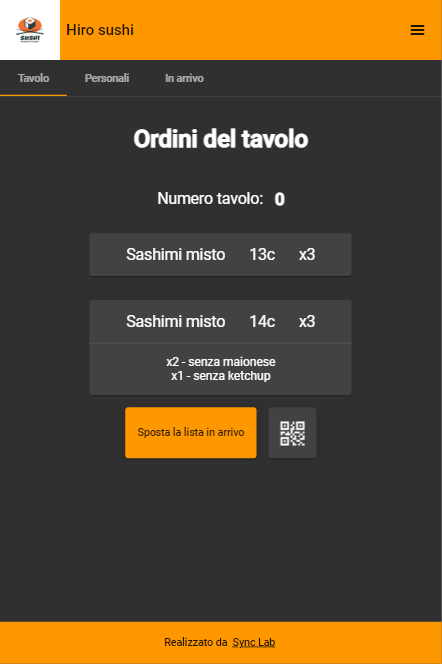
\includegraphics[scale=0.4]{ordinitavolo.png}
    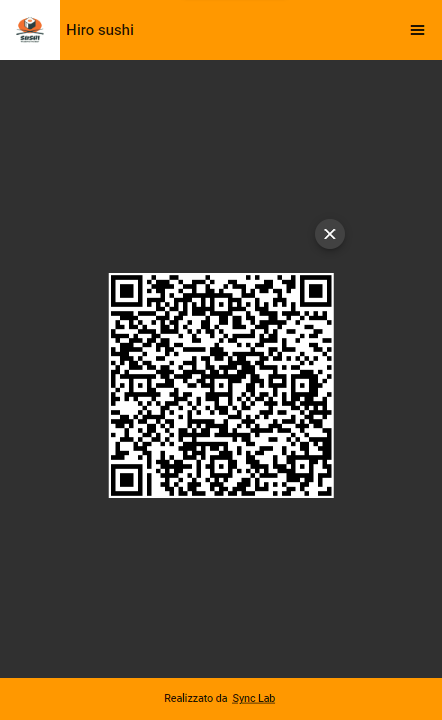
\includegraphics[scale=0.4]{ordinitavolo2.png}
    \caption{Maschera ordini del tavolo e QR-code degli ordini di SushiLab}
\end{figure}


\subsubsection{lista degli ordini personali}
Viene mostrata la lista degli ordini personali.\\
\textbf{Funzionalità:}
\begin{itemize}
    \item L'utente può visualizzare i piatti in modalità dettaglio;
    \item L'utente può visualizzare i piatti in modalità normale;
    \item L'utente può aggiungere un piatto nella lista dei preferiti o rimuoverlo dalla lista;
    \item L'utente può dare una recensione ad un piatto.
\end{itemize}
\begin{figure}[H]
    \centering
    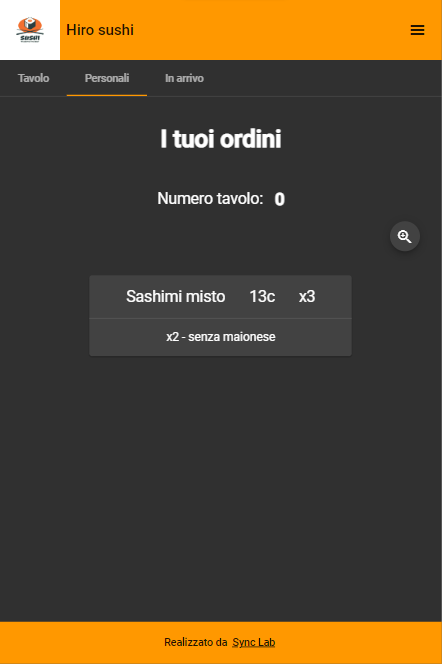
\includegraphics[scale=0.4]{ordinipersonali.png}
    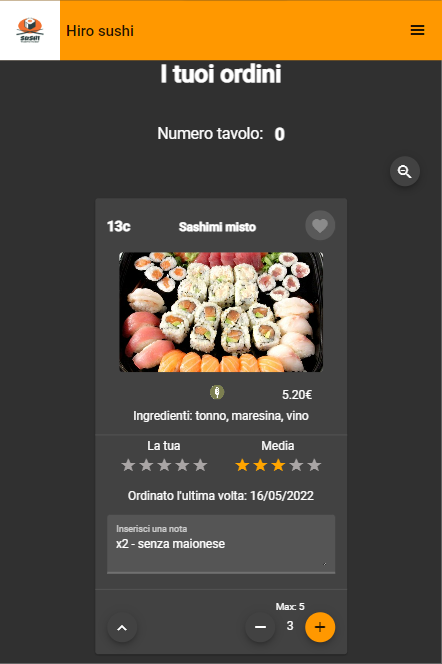
\includegraphics[scale=0.4]{ordinipersonali2.png}
    \caption{Maschera ordini personali di SushiLab}
\end{figure}


\subsubsection{lista degli ordini in arrivo}
Viene mostrata la lista degli ordini in arrivo.\\
\textbf{Funzionalità:}
\begin{itemize}
    \item L'utente può visualizzare i piatti in modalità dettaglio;
    \item L'utente può visualizzare i piatti in modalità normale;
    \item L'utente può marcare un piatto come arrivato;
    \item L'utente può aggiungere un piatto nella lista dei preferiti o rimuoverlo dalla lista;
    \item L'utente può dare una recensione ad un piatto.
\end{itemize}
\begin{figure}[H]
    \centering
    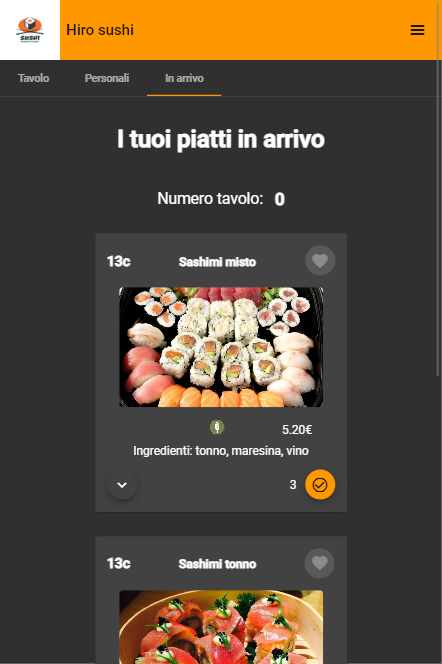
\includegraphics[scale=0.4]{ordiniinarrivo.png}
    \caption{Maschera ordini in arrivo di SushiLab}
\end{figure}


\subsubsection{Login}
Viene mostrato il form per effettuare il login dove è possibile effettuare la login nella piattaforma.\\
\textbf{Funzionalità:}
\begin{itemize}
    \item L'utente può effettuare il login inserendo i campi correttamente altrimenti viene evidenziato in rosso i campi sbagliati;
    \item L'utente può andare al form di registrazione;
    \item L'utente può andare al form di password dimenticata.
\end{itemize}
\begin{figure}[H]
    \centering
    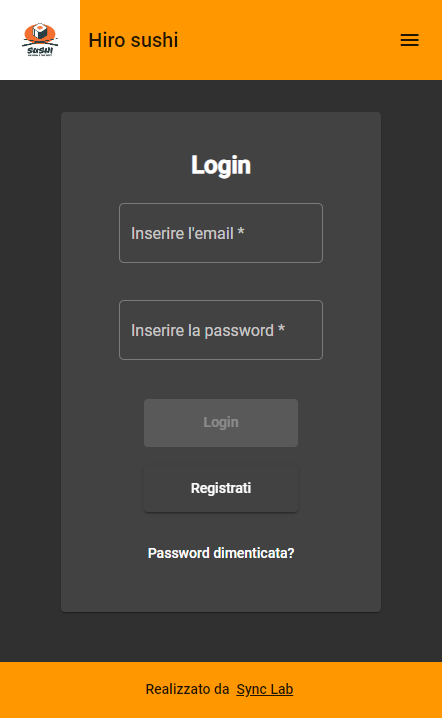
\includegraphics[scale=0.4]{login.png}
    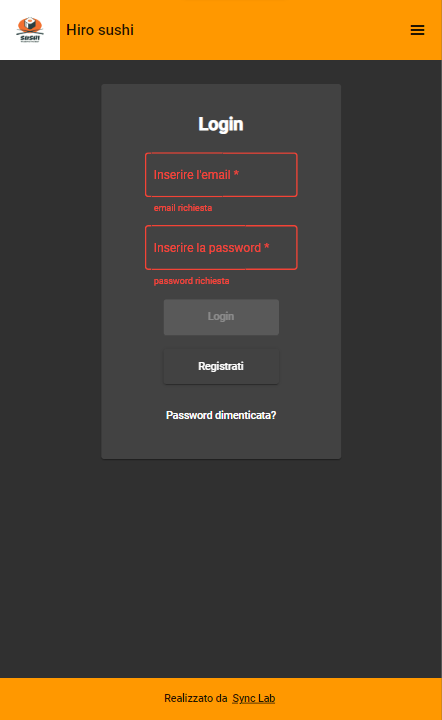
\includegraphics[scale=0.4]{login2.png}
    \caption{Maschera login di SushiLab}
\end{figure}


\subsubsection{Registrazione}
Viene mostrato il form di registrazione dove è possibile registrare nella piattaforma.\\
\textbf{Funzionalità:}
\begin{itemize}
    \item L'utente può effettuare la registrazione inserendo i campi correttamente altrimenti viene evidenziato in rosso i campi sbagliati;
    \item L'utente può andare al form di login.
\end{itemize}
\begin{figure}[H]
    \centering
    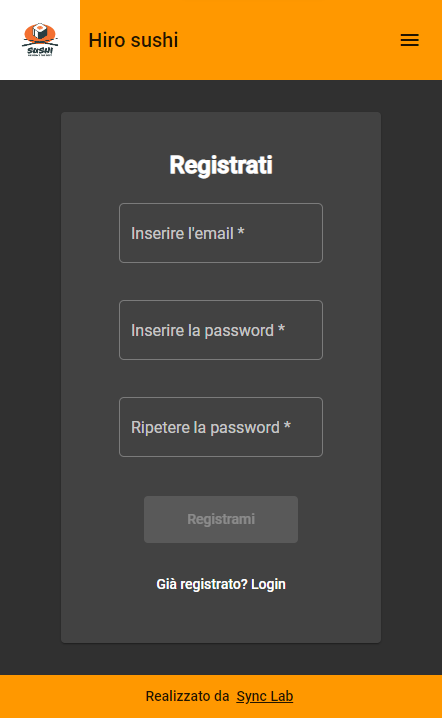
\includegraphics[scale=0.4]{registrati.png}
    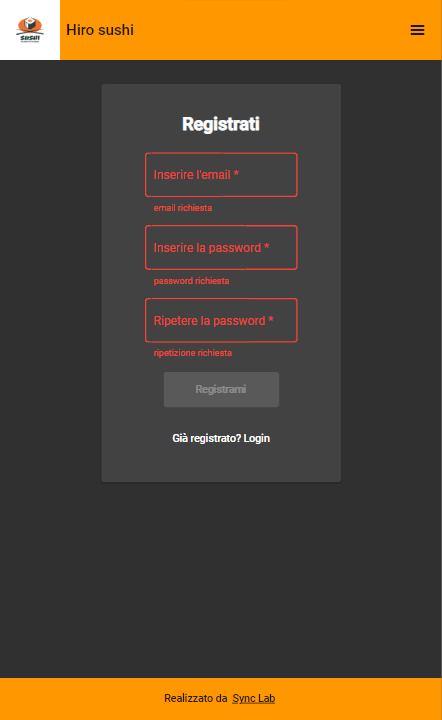
\includegraphics[scale=0.4]{registrati2.png}
    \caption{Maschera registrazione di SushiLab}
\end{figure}


\subsubsection{Password Dimenticata}
Viene mostrato il form di cambia password dove è possibile reimpostare la password.\\
\textbf{Funzionalità:}
\begin{itemize}
    \setlength\itemsep{.1em}
    \item L'utente può reimpostare la password inserendo i campi correttamente altrimenti viene evidenziato in rosso i campi sbagliati;
    \item L'utente può andare al form di registrazione;
    \item L'utente può andare al form di Login.
\end{itemize}
\begin{figure}[H]
    \centering
    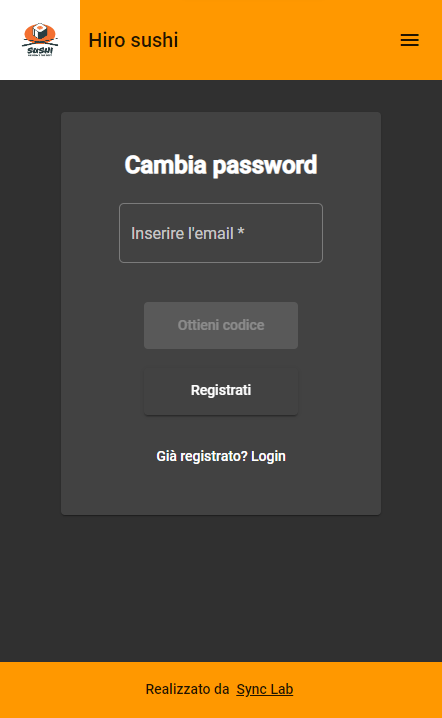
\includegraphics[scale=0.4]{cambiapass.png}
    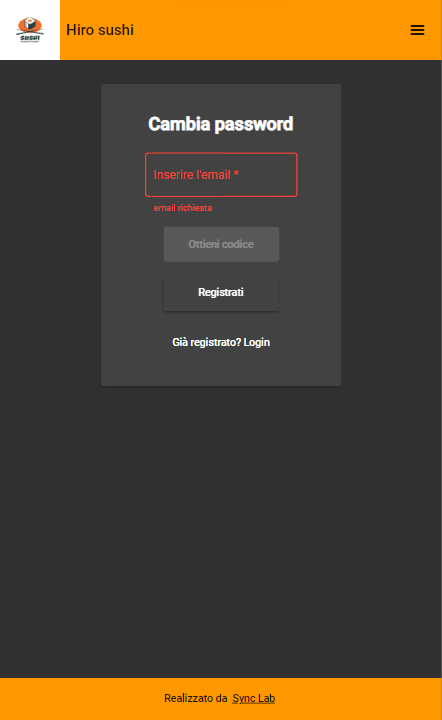
\includegraphics[scale=0.4]{cambiapass2.png}
    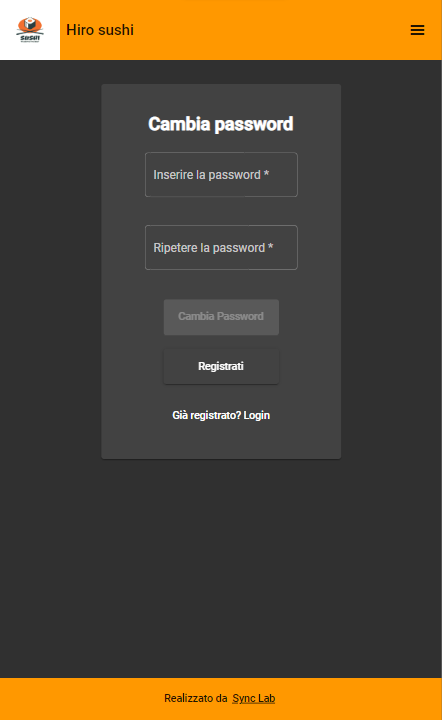
\includegraphics[scale=0.4]{cambiapass3.png}
    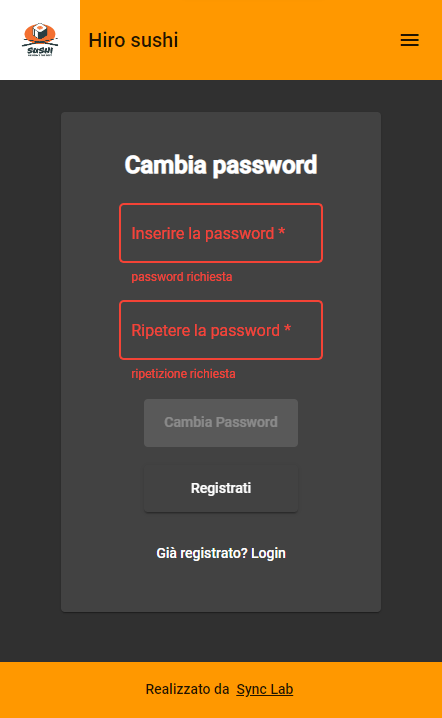
\includegraphics[scale=0.4]{cambiapass4.png}
    \caption{Maschere cambia password di SushiLab}
\end{figure}


\subsubsection{Area Personale}
Viene mostrata l'area personale dell'utente dove si può vedere i dati dell'utente.
\textbf{Funzionalità:}
\begin{itemize}
    \item L'utente può effettuare il logout;
    \item L'utente può andare nella sezione di blacklist degli ingredienti per inserire o rimuovere delle allergeni o preferenze.
\end{itemize}
\begin{figure}[H]
    \centering
    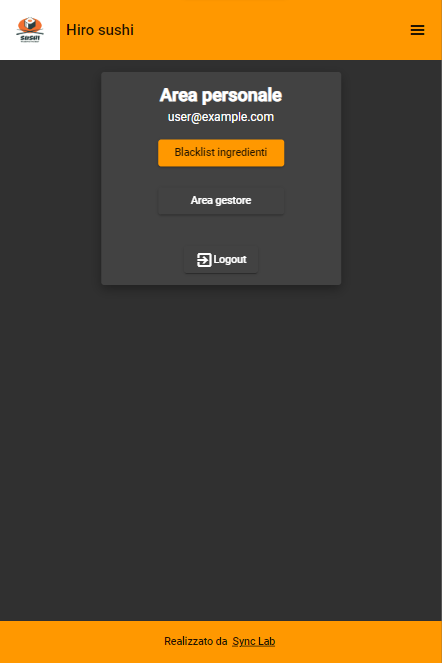
\includegraphics[scale=0.4]{personale.png}
    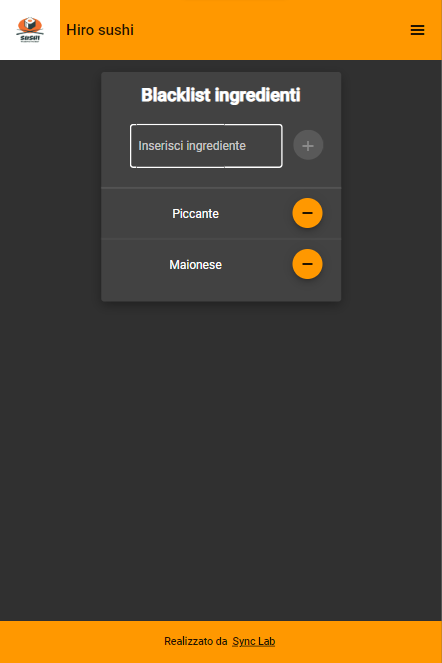
\includegraphics[scale=0.4]{blacklist.png}
    \caption{Maschera area personae e blacklist di SushiLab}
\end{figure}
\label{cap:menu.component}

\subsubsection{Menu component}
Componente usato per creare la maschera del menù. Composto da un insieme di piatti creati aumaticamenti in base al array menù di ritorno.\\
\textbf{Componenti e servizi usati:}
\begin{itemize}
    \item piatto.component;
    \item menu.service;
    \item ordini.service.
\end{itemize}

\subsubsection{Nav component}
Componente usato per creare la maschera della navbar. Composto da un insieme di link che porta l'utente in vari sezioni della web-app.\\
\textbf{Metodi:}
\begin{itemize}
    \item isLoggedIn(): ritorna true se l'utente è loggato, false altrimenti;
    \item haveMenu(): ritorna true se è presente il menù nel local storage, false altrimenti;
    \item haveTable(): ritorna true se è presente la sessione di tavole nel local storage, false altrimenti;
    \item close(): chiude il menu a tendina.
\end{itemize}
\textbf{Componenti e servizi usati:}
\begin{itemize}    
    \item auth.service;
    \item menu.service;
    \item table.service.
\end{itemize}

\subsubsection{Ordini component}
Componente usato per creare la maschera della lista degli ordini. Composto da tre sezioni che sono ordini del tavolo, ordini personali e ordini in arrivo.\\
\textbf{Metodi:}
\begin{itemize}
    \item moveOrders(): sposta la lista degli ordini del tavolo in arrivo;
    \item changeZoom(): cambia la modalità di presentazione dei piatti, cambiando da modificata normale in modificata dettaglio o viceversa;
    \item showQrCode(): mostra il QR-code della lista degli ordini;
    \item closeQrCode(): chiude la maschera di QR-code;
    \item getAllOrders(): inizializza tutti gli ordini predendo i piatti dal server.
\end{itemize}
\textbf{Componenti e servizi usati:}
\begin{itemize}
    \item piatto-arrivo.component;
    \item piatto.component;
    \item piatto-ordine.component;
    \item auth.service;
    \item menu.service;
    \item table.service.
\end{itemize}

\subsubsection{Piatto-arrivo component}
Componente usato per creare il piatto della sezione lista degli ordini in arrivo.\\
\textbf{Metodi:}
\begin{itemize}
    \item toogleFav(): cambia lo stato di preferito di un determinato piatto;
    \item updateStar(): aggiorna la recensione di un determinato piatto;
    \item decreaseCount(): chiamato quando utente marca un piatto come arrivato, diminuisce la quantità di un piatto in arrivo.
\end{itemize}
\textbf{Componenti e servizi usati:}
\begin{itemize}
    \item auth.service;
    \item menu.service.
\end{itemize}

% \subsubsection{Piatto-dettaglio component}
% Componente usato per creare il piatto in modalità dettaglio.\\
% \textbf{Metodi:}
% \begin{itemize}
%     \item toogleFav(): cambia lo stato di preferito di un determinato piatto;
%     \item updateStar(): aggiorna la recensione di un determinato piatto;
%     \item increseCount(): aumenta la quantità di un determinato piatto presente negli ordini personali;
%     \item decreaseCount(): diminuisce la quantità di un determinato piatto presente negli ordini personali
%     \item noteChanged(): cambia la nota di un piatto presente negli ordini personali.
% \end{itemize}
% \textbf{Componenti e servizi usati:}
% \begin{itemize}
%     \item auth.service;
%     \item ordini.service;
%     \item menu.service.
% \end{itemize}

\subsubsection{Piatto-ordine component}
Componente usato per creare il piatto in modalità normale per la sezione ordini dove viene mostrato solamente il nome, numero, quantità e la nota.\\

\subsubsection{Personale component}
Componente usato per creare la maschera dell'area personale, dove si può vedere email dell'utente e andare nella sezione blacklist.\\
\textbf{Metodi:}
\begin{itemize}
    \item isLoggedOut(): ritorna true se l'utente non è loggato, false altrimenti.
\end{itemize}
\textbf{Componenti e servizi usati:}
\begin{itemize}
    \item blacklist.component;
    \item forgot.component;
    \item login.component;
    \item logout.component;
    \item register.component;
    \item auth.service;
    \item user.service.
\end{itemize}

\subsubsection{blacklist component}
Componente usato per creare gestire la sezione blacklist degli ingredienti, viene mostrato la blacklist ed è possibile rimuovere o aggiungere un ingrediente.\\
\textbf{Metodi:}
\begin{itemize}
    \item onAdd(): metodo chiamato quando si aggiunge un ingrediente nella blacklist;
    \item onRemove(): metodo chiamato quando si rimuove un ingrediente dalla blacklist;
    \item isValid(): ritorna true se ingrediente inserito è valido, false altrimenti.
\end{itemize}
\textbf{Componenti e servizi usati:}
\begin{itemize}
    \item user.service.
\end{itemize}

\subsubsection{Forgot component}
Componente usato per creare la maschera per reimpostare la password.\\
\textbf{Metodi:}
\begin{itemize}
    \item sendCode(): chiama il server per mandare il link dove porta l'utente alla pagina per reimpostare la password;
    \item cambia(): metodo chiamato quando l'utente conferma il form, viene controllato i dati inseriti e in fine viene chiamato API per cambiare la password.
\end{itemize}
\textbf{Componenti e servizi usati:}
\begin{itemize}
    \item user.service.
\end{itemize}

\subsubsection{Login component}
Componente usato per creare la il form per effettuare la login.\\
\textbf{Metodi:}
\begin{itemize}
    \item login(): metodo chiamato quando l'utente conferma il form, viene controllato vari campi e infine viene chiamato API per effettuare la login.
\end{itemize}
\textbf{Componenti e servizi usati:}
\begin{itemize}
    \item auth.service.
\end{itemize}

\subsubsection{Logout component}
Componente usato per creare il bottone di logout e serve per effettuare il logout.\\
\textbf{Metodi:}
\begin{itemize}
    \item logout(): effettua il logout dell'utente.
\end{itemize}
\textbf{Componenti e servizi usati:}
\begin{itemize}
    \item auth.service.
\end{itemize}

\subsubsection{Register component}
Componente usato per creare il form per la registrazione.\\
\textbf{Metodi:}
\begin{itemize}
    \item register(): metodo chiamato quando l'utente conferma il form, viene controllato vari campi e infine viene chiamato API per la registrazione.
\end{itemize}
\textbf{Componenti e servizi usati:}
\begin{itemize}
    \item user.service.
\end{itemize}

\subsubsection{Preferiti component}
Componente usato per creare la maschera dei preferiti dove si può visualizzare la lista dei preferiti e rimuovere un piatto non più interessante.\\
\textbf{Componenti e servizi usati:}
\begin{itemize}
    \item piatto.component;
    \item menu.service.
\end{itemize}

\subsubsection{Piatto component}
Componente usato per creare il piatto, viene utilizzato per la visualizzazione del menù e della lista dei preferiti.\\
\textbf{Componenti e servizi usati:}
\begin{itemize}
    \item menu.service.
\end{itemize}

\subsubsection{Preferiti component}
Componente usato per creare la maschera dei preferiti dove si può visualizzare la lista dei preferiti e rimuovere un piatto non più interessante.\\
\textbf{Metodi:}
\begin{itemize}
    \item toggleExpand(): espande la visuale del piatto mostrando tutti i dettagli del piatto o nasconde i suoi dettagli;
    \item toogleFav(): cambia lo stato di preferito di un determinato piatto;
    \item updateStar(): aggiorna la recensione di un determinato piatto;
    \item increseCount(): aumenta la quantità di un determinato piatto presente negli ordini personali;
    \item decreaseCount(): diminuisce la quantità di un determinato piatto presente negli ordini personali
    \item noteChanged(): cambia la nota di un piatto presente negli ordini personali.
\end{itemize}
\textbf{Componenti e servizi usati:}
\begin{itemize}
    \item star.component;
    \item ordini.service;
    \item auth.service;
    \item menu.service.
\end{itemize}

\subsubsection{Tavolo component}
Componente usato per creare la maschera gestione del tavolo, dove si può creare una sessione di tavolo, unire ad una sessione o uscire da una sessione.\\
\textbf{Metodi:}
\begin{itemize}
    \item changeState(): cambia lo stato di visualizzazione della sezione gestione del tavolo in base al table.service se è presente o no una sessione;
    \item removeSession(): rimuove la sessione del tavolo;
    \item setSession(): imposta la sessione del tavolo chiamando il server e infine imposta il numero di tavolo;
    \item updateURL(): aggiorna il percorso del link per generare il QR-code del tavolo;
    \item createSession(): crea la sessione di tavolo.
\end{itemize}
\textbf{Componenti e servizi usati:}
\begin{itemize}
    \item table.service;
    \item menu.service.
\end{itemize}

\subsubsection{auth.service}
Servizio utilizzato per gestire le autenticazioni.
\textbf{Metodi:}
\begin{itemize}
    \item login(email: string, password: string): metodo chiamato per effettuare la login dell'utente;
    \item setSession(): salva i dati dell'utente dopo la login nel local storage per mantenere la sessione di login;
    \item logout(): metodo chiamato per effettuare il logout dell'utente;
    \item isLoggedIn(): ritorna true se è presente nel local storage la sessione dell'utente, false altrimenti;
    \item getExpirations(): ritorna true se la sessione dell'utente non è ancora scaduto, false altrimenti.
\end{itemize}

\subsubsection{menu.service}
Servizio utilizzato per gestire tutte le funzionalità del menù.\\
\textbf{Metodi:}
\begin{itemize}
    \item title(): ritorna il nome del menù;
    \item haveMenu(): ritorna true se è presente un menù nel local storage, false altrimenti;
    \item get menuId(): ritorna l'id del menù;
    \item set menuId(id: number): salva l'id del menù nel local storage;
    \item applyBlacklist(menu: Menu): rimuove i piatti che contengono gli ingredienti presenti nella blacklist dell'utente;
    \item setFavorite(idPiatto:number, favorite:boolean): aggiunge un piatto del menù nella lista dei preferiti o lo toglie dalla lista dei preferiti;
    \item  setRating(idPiatto: number, rate: number): salva la recensione del piatto;
    \item getPreferiti(): richiede al server la lista dei preferiti dell'utente.
\end{itemize}

\subsubsection{ordini.service}
Servizio utilizzato per gestire le ordinazioni.\\
\textbf{Metodi:}
\begin{itemize}
    \item updateRemoteOrder(): aggiorna gli ordini del server mandandogli la lista degli ordini ogni lasso di tempo;
    \item getOrded(idPiatto:number): ritorna indice nel array di ordini del piatto passato;
    \item clearOrder(): svuota array di ordini presente nel local storage;
    \item setOrder(idPiatto: number, count: number, note: string): imposta la quantità del piatto  con id idPiatto passato presente nalla lista degli ordini con count;
    \item mergeOrder(newOrders: any[]): unisce gli ordini locali con quelli del server quando l'utente si unisce ad una sessione passando da una sessione a una sessione diversa;
    \item getSessionCode(): ritorna il codice sessione del tavolo;
    \item getOrdersTable(): ritorna l'ordine del tavolo;
    \item getOrdersUser(): ritorna l'ordine dell'utente;
    \item getOrdersArriving(): ritorna l'ordine in arrivo;
    \item moveOrders(): sposta l'ordine del tavolo in arrivo;
    \item toQrCode(): ritorna la stringa per generare il qrcode per la lista dell'ordine.
\end{itemize}

\subsubsection{tavolo.service}
Servizio utilizzato per gestire le sessioni di tavolo.\\
\textbf{Metodi:}
\begin{itemize}
    \item createSession(): chiama il server per creare una sessione di tavolo;
    \item getSession(): ritorna il numero del tavolo;
    \item getCode(): ritorna il codice di sessione;
    \item haveSession(): ritorna true se esiste un codice di sessione false altrimenti;
    \item setSession(code: string): imposta il codice di sessione con il code passato come parametro per unirsi alla sessione del tavolo;l
    \item menuChanged(): controlla se il menu della sessione corrente è uguale a quello della sessione a cui si vuole unirsi se è false non è possibile fare il merge dei piatti;
    \item removeSession(): rimuove i dati della sessione di tavolo.
\end{itemize}


\subsubsection{user.service}
Servizio utilizzato per gestire le funzionalità dell'area personale.\\
\textbf{Metodi:}
\begin{itemize}
    \item pushBlacklist(): chiama il server aggiornare la blacklist degli ingredienti;
    \item getUtente(): richiede al server per ottenere le informazione dell'utente attualmente collegato;
    \item setUtente(user: User): manda al server i dati dell'utente per completare la registrazione;
    \item verifyCode(code: string): verifica se il link con cui è passato al form per reimpostare la password è corretto o no;
    \item getChangeCod(email: string): chiede al server per mandare un'email per al email passato per reimpostare la password;
    \item changePassword(password: string): manda al server la password nuova per aggiornare quella vecchia.
\end{itemize}